\section{Appendix A: Effect of the Losses}
\label{sect:app_ablations}
Table~\ref{tab:ablations} gives the values and significance tests behind Fig.~\ref{fig:q2}.
\begin{table}[t]
\centering
\caption{Effect of the PET and rigidity losses on the test set (CT Dice: 28 patients, 38 pairs; PET: 26 patients, 30 pairs). Each network is trained with the given losses and evaluated as is (left) and with instance optimisation (IO) using the same losses (right). Mean$\pm$SD over patients. $^{\dagger}$/$^{\ddagger}$: significantly better/worse than ``Neither'' in the same block (two-sided Wilcoxon signed-rank test on patient values, Holm-corrected over three comparisons within each column, $p<0.05$).}
\label{tab:ablations}
\scriptsize
\setlength{\tabcolsep}{3pt}
\begin{tabular}{lcccccc}
\toprule
 & \multicolumn{3}{c}{Network} & \multicolumn{3}{c}{Network + IO} \\
\cmidrule(lr){2-4} \cmidrule(lr){5-7}
Losses & Dice (\%) $\uparrow$ & $|\Delta\mathrm{MTV}|$ (\%) $\downarrow$ & $|\Delta\mathrm{TLG}|$ (\%) $\downarrow$ & Dice (\%) $\uparrow$ & $|\Delta\mathrm{MTV}|$ (\%) $\downarrow$ & $|\Delta\mathrm{TLG}|$ (\%) $\downarrow$ \\
\midrule
Neither & 74.8$\pm$4.5 & 10.6$\pm$10.2 & 10.8$\pm$11.7 & 79.2$\pm$4.3 & 10.2$\pm$10.1 & 11.9$\pm$12.5 \\
PET & 72.9$\pm$4.4$^{\ddagger}$ & 7.6$\pm$9.0$^{\dagger}$ & 7.6$\pm$9.3$^{\dagger}$ & 76.4$\pm$4.7$^{\ddagger}$ & 6.3$\pm$9.1$^{\dagger}$ & 7.2$\pm$9.4$^{\dagger}$ \\
Rigidity & 74.8$\pm$4.5 & 9.4$\pm$9.5$^{\dagger}$ & 9.5$\pm$10.9$^{\dagger}$ & 78.7$\pm$4.2$^{\ddagger}$ & 7.9$\pm$9.0$^{\dagger}$ & 10.1$\pm$11.0 \\
PET + rigidity & 72.8$\pm$4.3$^{\ddagger}$ & 7.4$\pm$9.0$^{\dagger}$ & 7.7$\pm$10.1$^{\dagger}$ & 75.6$\pm$4.8$^{\ddagger}$ & 6.2$\pm$8.7$^{\dagger}$ & 7.9$\pm$9.0 \\
\bottomrule
\end{tabular}
\end{table}


\section{Appendix B: Per-Lesion Uptake Change}
\label{sect:app_lesions_tlg}

\begin{figure}[t]
\centering
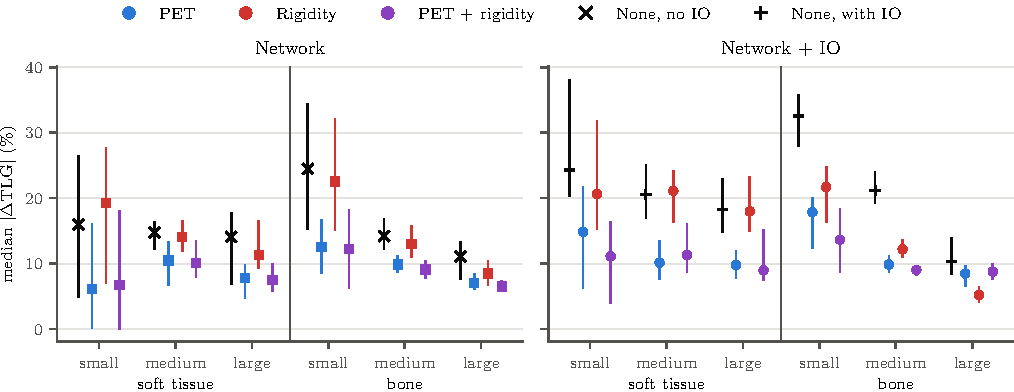
\includegraphics[width=\textwidth]{figures/lesions_tlg.pdf}
\caption{Per-lesion absolute total lesion glycolysis (TLG) change on the test set (1327 lesions from 26 patients and 30 pairs after excluding 108 components smaller than five voxels), stratified by location (soft tissue or bone-associated, with $\geq$50\,\% of the lesion on bone) and size (small $<0.5$~ml, medium $0.5$ to $<5$~ml, large $\geq5$~ml).
 Points show the median $|\Delta\mathrm{TLG}|$ per lesion; left: network output, right: instance optimization (IO) with the same losses.
 Within each size stratum, the loss groups are ordered PET, rigidity, and PET plus rigidity; squares and circles denote without and with IO, while $\times$ and $+$ denote the corresponding configurations without losses.
 Error bars: 95\,\% confidence intervals from a patient-cluster bootstrap.}
\label{fig:lesions_tlg}
\end{figure}


\section{Appendix C: Tuning of Instance Optimisation}
\label{sect:app_io_tuning}
Table~\ref{tab:io_tuning} lists all candidates of the two IO tuning stages on the validation set (Sec.~\ref{sect:tuning}) and the selected settings.
\begin{table}[t]
\centering
\caption{Instance-optimization (IO) tuning on the validation set (CT Dice: 26 patients, 38 pairs; metabolic tumor volume [MTV] and total lesion glycolysis [TLG]: 26 patients, 32 lesion-positive pairs), using the network trained with the PET-preservation and rigidity losses.
 Stage 1 varies learning rate and iterations; stage 2 varies the common scale of the four PET weights relative to the training-derived values.
 Within each stage, the chosen setting (bold) has the lowest $|\Delta\mathrm{MTV}|+|\Delta\mathrm{TLG}|$ among candidates within two Dice points of the most accurate one (``Within'').
 Candidates are sorted by Dice; values are means over patients after averaging eligible pairs; the rigidity weight was fixed at 0.25 (Sec.~\ref{sect:tuning}).}
\label{tab:io_tuning}
\resizebox{\textwidth}{!}{%
\begin{tabular}{lccccccc}
\toprule
Candidate & Dice (\%) & HD95 (mm) & $|\Delta\mathrm{MTV}|$ (\%) & $|\Delta\mathrm{TLG}|$ (\%) & Sum (\%) & NDV (ppm) & Within \\
\midrule
\multicolumn{8}{l}{\textit{Stage 1: learning rate / iterations}} \\
0.1 / 20 & 78.7 & 6.58 & 10.0 & 9.8 & 19.8 & 15 & yes \\
0.1 / 40 & 78.6 & 6.58 & 10.9 & 10.6 & 21.5 & 13 & yes \\
0.1 / 10 & 78.1 & 6.69 & 7.6 & 8.4 & 16.0 & 17 & yes \\
0.05 / 40 & 78.0 & 6.78 & 6.9 & 8.1 & 15.0 & 29 & yes \\
0.05 / 20 & 77.8 & 6.81 & 6.7 & 8.0 & 14.7 & 29 & yes \\
0.05 / 10 & 77.0 & 6.84 & 5.3 & 7.0 & 12.2 & 34 & yes \\
\textbf{0.025 / 40} & 77.0 & 6.89 & 4.6 & 6.2 & 10.7 & 12 & yes \\
0.025 / 20 & 76.7 & 6.93 & 4.6 & 6.3 & 10.9 & 12 & yes \\
0.0125 / 40 & 76.1 & 6.99 & 3.9 & 5.7 & 9.6 & 2 & no \\
0.025 / 10 & 75.7 & 7.14 & 4.3 & 5.5 & 9.8 & 18 & no \\
0.0125 / 20 & 75.6 & 7.16 & 3.6 & 5.1 & 8.7 & 2 & no \\
0.0125 / 10 & 75.3 & 7.17 & 3.2 & 4.6 & 7.8 & 3 & no \\
\midrule
\multicolumn{8}{l}{\textit{Stage 2: PET weight scale (learning rate 0.025, 40 iterations)}} \\
$\times$0 & 79.5 & 6.61 & 10.1 & 11.5 & 21.6 & 0 & yes \\
\textbf{$\times$0.1} & 77.9 & 6.77 & 5.6 & 7.8 & 13.4 & 7 & yes \\
$\times$0.25 & 77.1 & 6.86 & 5.1 & 6.8 & 11.9 & 12 & no \\
$\times$0.5 & 77.1 & 6.87 & 4.9 & 6.6 & 11.5 & 12 & no \\
$\times$1 & 77.1 & 6.87 & 5.0 & 6.7 & 11.6 & 12 & no \\
$\times$2 & 77.0 & 6.89 & 4.9 & 6.6 & 11.5 & 13 & no \\
$\times$4 & 77.0 & 6.89 & 4.6 & 6.2 & 10.8 & 12 & no \\
\bottomrule
\end{tabular}}
\end{table}


\section{Appendix D: Signed Change of Lesion Volume and Uptake}
\label{sect:app_signed}
The main results report the absolute change of MTV and TLG.
Table~\ref{tab:signed} gives the signed change, which shows whether a method systematically enlarges or shrinks the lesions.
Every method enlarged the lesions on average (mean $\Delta\mathrm{MTV}$ $+1.1$ to $+8.2$\,\%, $\Delta\mathrm{TLG}$ $+2.8$ to $+9.6$\,\%), including the affine pre-registration ($+2.9$\,\% and $+2.8$\,\%); the spread over patients was larger than these means for every deformable method.
\begin{table}[t]
\centering
\caption{Signed change in metabolic tumor volume (MTV) and total lesion glycolysis (TLG) caused by registration on the test set (26 patients, 30 lesion-positive pairs): positive values mean that the warped lesions are larger or have greater total uptake.
 Methods are as in Table~\ref{tab:baselines}; Training / IO indicates where losses are used, and PET + rig. denotes PET-preservation and rigidity losses.
 Values are mean$\pm$SD and median over patients after averaging each patient's eligible pairs.}
\label{tab:signed}
\small
\begin{tabular}{lllcccc}
\toprule
 & & & \multicolumn{2}{c}{$\Delta\mathrm{MTV}$ (\%)} & \multicolumn{2}{c}{$\Delta\mathrm{TLG}$ (\%)} \\
\cmidrule(lr){4-5}\cmidrule(lr){6-7}
Method & Training & IO & Mean$\pm$SD & Median & Mean$\pm$SD & Median \\
\midrule
Affine & -- & -- & $+2.9\pm5.8$ & $+1.3$ & $+2.8\pm5.7$ & $+1.7$ \\
NiftyReg & -- & -- & $+4.6\pm14.7$ & $+0.5$ & $+6.3\pm18.7$ & $+0.3$ \\
ConvexAdam & -- & -- & $+8.2\pm12.8$ & $+5.8$ & $+9.6\pm17.2$ & $+5.7$ \\
Affine + IO & -- & PET + rig. & $+3.5\pm5.8$ & $+3.8$ & $+5.7\pm5.6$ & $+6.7$ \\
\midrule
Ours & -- & -- & $+5.3\pm13.1$ & $+4.5$ & $+7.9\pm14.9$ & $+7.0$ \\
Ours & PET + rig. & -- & $+5.1\pm11.0$ & $+3.4$ & $+7.6\pm12.5$ & $+5.2$ \\
Ours + IO & -- & basic & $+1.1\pm16.5$ & $+2.1$ & $+4.0\pm20.0$ & $+3.6$ \\
Ours + IO & PET + rig. & PET + rig. & $+4.2\pm11.8$ & $+3.0$ & $+7.3\pm12.8$ & $+6.4$ \\
Ours + IO & -- & PET + rig. & $+3.2\pm13.5$ & $+3.1$ & $+6.2\pm14.8$ & $+6.2$ \\
\bottomrule
\end{tabular}
\end{table}


\section{Appendix E: Lesion Coverage in Predicted Masks}
\label{sect:app_detection}
Tables~\ref{tab:detection_groups} and~\ref{tab:detection_contributions} give the numbers behind Fig.~\ref{fig:detection}.
\begin{table}[t]
\centering
\caption{Volume and uptake change of ground-truth lesions, grouped by how much of each lesion the predicted lesion mask seen by IO covers (test set; network trained without PET losses, IO with the PET weights scaled by the given factor). Per scan, the change of the summed volume or uptake of the group's lesions relative to the unwarped moving scan, in \%; mean over the patients with lesions in the group.}
\label{tab:detection_groups}
\scriptsize
\setlength{\tabcolsep}{3pt}
\begin{tabular}{lcccccc}
\toprule
 & \multicolumn{2}{c}{Missed} & \multicolumn{2}{c}{Partly ($<$50\,\%)} & \multicolumn{2}{c}{Covered ($\geq$50\,\%)} \\
 & \multicolumn{2}{c}{\tiny 214 lesions, 6\,\% of volume} & \multicolumn{2}{c}{\tiny 155 lesions, 6\,\% of volume} & \multicolumn{2}{c}{\tiny 1066 lesions, 88\,\% of volume} \\
\cmidrule(lr){2-3}\cmidrule(lr){4-5}\cmidrule(lr){6-7}
 & $|\Delta\mathrm{MTV}|$ & $|\Delta\mathrm{TLG}|$ & $|\Delta\mathrm{MTV}|$ & $|\Delta\mathrm{TLG}|$ & $|\Delta\mathrm{MTV}|$ & $|\Delta\mathrm{TLG}|$ \\
\midrule
Network only & 14.9 & 16.4 & 12.0 & 13.5 & 7.4 & 6.9 \\
\midrule
+ IO, PET $\times$0 & 14.9 & 17.0 & 11.3 & 14.6 & 7.8 & 7.9 \\
+ IO, PET $\times$0.1 (tuned) & 15.7 & 17.3 & 11.5 & 12.7 & 4.9 & 5.1 \\
+ IO, PET $\times$1 & 15.5 & 17.3 & 11.4 & 12.7 & 4.9 & 5.1 \\
\bottomrule
\end{tabular}
\end{table}

\begin{table}[t]
\centering
\caption{Contribution of all 1435 provided lesion components in 26 test patients (30 pairs), grouped by how much of each component the predicted lesion mask used by instance optimization (IO) covers, to the evaluated metabolic tumor volume (MTV) and total lesion glycolysis (TLG) change; the network is trained without PET losses and IO uses the PET weights scaled by the stated factor.
 Contribution of a group: the change per image if only the group's lesions changed and all other lesions kept their volume and uptake, in \%; mean over patients.
 All: the evaluation metric.
 Since changes of different lesions in an image partly cancel, the contributions add up to slightly more.}
\label{tab:detection_contributions}
\scriptsize
\setlength{\tabcolsep}{3pt}
\begin{tabular}{lcccccccc}
\toprule
 & \multicolumn{2}{c}{Missed} & \multicolumn{2}{c}{Partly ($<$50\,\%)} & \multicolumn{2}{c}{Covered ($\geq$50\,\%)} & \multicolumn{2}{c}{All lesions} \\
 & \multicolumn{2}{c}{\tiny 214 lesions, 6\,\% of volume} & \multicolumn{2}{c}{\tiny 155 lesions, 6\,\% of volume} & \multicolumn{2}{c}{\tiny 1066 lesions, 88\,\% of volume} & \multicolumn{2}{c}{\tiny 1435 lesions} \\
\cmidrule(lr){2-3}\cmidrule(lr){4-5}\cmidrule(lr){6-7}\cmidrule(lr){8-9}
 & $|\Delta\mathrm{MTV}|$ & $|\Delta\mathrm{TLG}|$ & $|\Delta\mathrm{MTV}|$ & $|\Delta\mathrm{TLG}|$ & $|\Delta\mathrm{MTV}|$ & $|\Delta\mathrm{TLG}|$ & $|\Delta\mathrm{MTV}|$ & $|\Delta\mathrm{TLG}|$ \\
\midrule
Network only & 4.6 & 5.4 & 1.3 & 1.0 & 5.2 & 6.5 & 10.3 & 12.5 \\
\midrule
+ IO, PET $\times$0 & 5.3 & 6.4 & 1.3 & 1.2 & 5.3 & 7.3 & 11.3 & 14.5 \\
+ IO, PET $\times$0.1 (tuned) & 5.2 & 6.2 & 1.4 & 1.0 & 3.3 & 5.4 & 9.3 & 11.8 \\
+ IO, PET $\times$1 & 5.3 & 6.3 & 1.1 & 0.8 & 3.3 & 5.1 & 9.0 & 11.5 \\
\bottomrule
\end{tabular}
\end{table}


\section{Appendix F: Rigidity Penalties}
\label{sect:app_rigidity}
Table~\ref{tab:rigidity_full} lists all measures of the rigidity comparison, including the three terms of the Staring energy, HD95, and folding in and around the bones.
\begin{table}[t]
\centering
\caption{All measures of the rigidity comparison on the test set (alignment and rigidity: 28 patients, 38 pairs; PET preservation: 26 patients, 30 pairs), using the network trained with the PET losses followed by instance optimization (IO) with the PET terms and one rigidity penalty at the weight chosen on the validation set.
 Rigidity of bones: residual of a rigid fit to each bone (minimized by the rigid-fit penalty), Staring energy (minimized by the Staring penalty), and distortion of short (5--15~mm) and long ($\geq$15~mm) within-bone distances (minimized by neither).
 HD95: 95th-percentile Hausdorff distance over bones and soft-tissue organs; near-bone soft tissue: soft-tissue organs within three voxels of a bone; Staring energy: sum of its properness, orthonormality, and affinity terms on the whole bone; NDV: non-diffeomorphic volume; NDV in bone band: in a three-voxel band around the bones.
 Mean$\pm$SD over patients; $^{\dagger}$/$^{\ddagger}$: significantly better/worse than without rigidity (two-sided Wilcoxon signed-rank test on patient values, Holm-corrected over the three penalties per row, $p<0.05$).}
\label{tab:rigidity_full}
\resizebox{\textwidth}{!}{%
\begin{tabular}{lcccc}
\toprule
Measure & No rigidity & Staring ($\times$3) & Staring + erosion ($\times$100) & Per-bone rigid fit ($\times$100) \\
\midrule
\multicolumn{5}{l}{\textit{Alignment}} \\
CT Dice (\%) & 77.7$\pm$4.8 & 75.7$\pm$4.3$^{\ddagger}$ & 77.6$\pm$4.6 & 76.1$\pm$4.6$^{\ddagger}$ \\
CT HD95 (mm) & 6.96$\pm$2.35 & 7.03$\pm$2.35$^{\ddagger}$ & 6.90$\pm$2.34 & 7.03$\pm$2.35 \\
Bone Dice (\%) & 78.4$\pm$6.4 & 74.6$\pm$5.7$^{\ddagger}$ & 77.5$\pm$6.2$^{\ddagger}$ & 74.5$\pm$6.2$^{\ddagger}$ \\
Bone HD95 (mm) & 7.53$\pm$3.38 & 7.68$\pm$3.40$^{\ddagger}$ & 7.54$\pm$3.36 & 7.79$\pm$3.41$^{\ddagger}$ \\
Soft-tissue Dice (\%) & 79.9$\pm$3.9 & 79.8$\pm$3.9 & 80.7$\pm$3.9$^{\dagger}$ & 80.8$\pm$4.0$^{\dagger}$ \\
Soft-tissue HD95 (mm) & 6.31$\pm$2.94 & 6.29$\pm$2.95 & 6.18$\pm$2.98$^{\dagger}$ & 6.18$\pm$3.01$^{\dagger}$ \\
Near-bone soft-tissue Dice (\%) & 74.1$\pm$4.3 & 73.7$\pm$4.2$^{\ddagger}$ & 74.9$\pm$4.2$^{\dagger}$ & 74.8$\pm$4.2 \\
\multicolumn{5}{l}{\textit{Rigidity of bones}} \\
Rigid-fit residual (mm) & 2.67$\pm$0.52 & 2.00$\pm$0.48$^{\dagger}$ & 2.31$\pm$0.47$^{\dagger}$ & 1.39$\pm$0.40$^{\dagger}$ \\
Staring energy & 3.517$\pm$2.110 & 0.272$\pm$0.090$^{\dagger}$ & 1.803$\pm$0.650$^{\dagger}$ & 1.419$\pm$0.473$^{\dagger}$ \\
Staring properness & 0.182$\pm$0.100 & 0.022$\pm$0.009$^{\dagger}$ & 0.097$\pm$0.033$^{\dagger}$ & 0.093$\pm$0.027$^{\dagger}$ \\
Staring orthonormality & 1.431$\pm$0.840 & 0.160$\pm$0.066$^{\dagger}$ & 0.765$\pm$0.289$^{\dagger}$ & 0.733$\pm$0.261$^{\dagger}$ \\
Staring affinity & 1.903$\pm$1.180 & 0.090$\pm$0.040$^{\dagger}$ & 0.942$\pm$0.339$^{\dagger}$ & 0.594$\pm$0.205$^{\dagger}$ \\
Distortion short (\%) & 13.41$\pm$3.62 & 5.53$\pm$1.04$^{\dagger}$ & 8.76$\pm$1.04$^{\dagger}$ & 5.01$\pm$1.13$^{\dagger}$ \\
Distortion long (\%) & 4.44$\pm$0.83 & 3.17$\pm$0.68$^{\dagger}$ & 3.53$\pm$0.63$^{\dagger}$ & 1.83$\pm$0.62$^{\dagger}$ \\
\multicolumn{5}{l}{\textit{Regularity}} \\
NDV (ppm) & 7.9$\pm$29.2 & 7.9$\pm$29.3$^{\dagger}$ & 0.7$\pm$0.6 & 0.6$\pm$0.6$^{\dagger}$ \\
NDV in bone (ppm) & 6.5$\pm$4.6 & 0.3$\pm$1.2$^{\dagger}$ & 16.5$\pm$23.6$^{\ddagger}$ & 9.6$\pm$23.7 \\
NDV in bone band (ppm) & 1.9$\pm$1.7 & 0.7$\pm$0.9$^{\dagger}$ & 3.7$\pm$4.0$^{\ddagger}$ & 3.6$\pm$4.6$^{\ddagger}$ \\
\multicolumn{5}{l}{\textit{Preservation}} \\
$|\Delta\mathrm{MTV}|$ (\%) & 8.2$\pm$10.1 & 7.1$\pm$8.7 & 7.9$\pm$10.0 & 8.0$\pm$8.9 \\
$|\Delta\mathrm{TLG}|$ (\%) & 10.3$\pm$10.2 & 9.2$\pm$9.4 & 9.6$\pm$10.2 & 10.5$\pm$9.4 \\
\bottomrule
\end{tabular}}
\end{table}

